%
% Optional reading
%

\begin{frame}[plain,c]
\begin{center}
{\Huge \bf Optional reading for Lecture \thislecture}
\end{center}
\end{frame}

% ------------------------------------------------------------------------------

%
% Worked example :
%

{
\problemslide

\begin{frame}{Worked example: Electric field and force of 3 point charges}

\begin{blockexmplque}{Question}
  Three charges are arranged as following:
  $Q_1$ = 1 nC at (-1,-1,0) cm, $Q_2$ = 1 nC at (1,-1,0) cm and $Q_3$ = -2nC at (0,2,0) cm.
  Calculate:
  \begin{enumerate}
    \item The electric field (vector) at the point (0,0,0).
    \item The force acting on charge $Q_3$.
  \end{enumerate}
\end{blockexmplque}

\vspace{0.2cm}

The electric field $\vec{E}$ at $\vec{r}$, due to $Q_1$, $Q_2$, and $Q_3$,
is given by the superposition of the fields produced by each point charge:
\begin{equation*}
  \vec{E}(\vec{r}) = \frac{1}{4\pi \epsilon_0}
       \sum_{i=1}^{2} \frac{Q_i}{|\vec{r}-\vec{r}_i|^3} \Big( \vec{r}-\vec{r}_i \Big)
\end{equation*}

Therefore, at $\vec{r}=\vec{0}$, it is given by:
\begin{equation*}
  \vec{E}(\vec{0}) = \frac{1}{4\pi \epsilon_0} \Big\{
          \frac{Q_1}{|\vec{r}_1|^3} \Big( - \vec{r}_1 \Big) +
          \frac{Q_2}{|\vec{r}_2|^3} \Big( - \vec{r}_2 \Big) +
          \frac{Q_3}{|\vec{r}_3|^3} \Big( - \vec{r}_3 \Big)
      \Big\}
\end{equation*}

\end{frame}

%
%
%

\begin{frame}{Worked example: Electric field and force of 3 point charges}

Substituting the given quantities into the previous equation, we get:
\begin{equation*}
  \vec{E}(\vec{0}) =
      (9.0 \times 10^9 \; \frac{N \cdot m^2}{C^2}) \Big\{
          \frac{ (1.0 \times 10^{-9} \; C)}{\sqrt{2}^3 \times 10^{-6} \; m^3} \Big( 1, 1, 0 \Big) \times 10^{-2} m +
\end{equation*}
\begin{equation*}
        + \frac{ (1.0 \times 10^{-9} \; C)}{\sqrt{2}^3 \times 10^{-6} \; m^3} \Big(-1, 1, 0 \Big) \times 10^{-2} m +
          \frac{(-2.0 \times 10^{-9} \; C)}{2^3 \times 10^{-6} \; m^3}        \Big( 0,-2, 0 \Big) \times 10^{-2} m
      \Big\} \Rightarrow
\end{equation*}

\begin{equation*}
  \vec{E}(\vec{0}) =
      9.0 \times 10^9 \Big\{
          \frac{2.0 \times 10^{-11}}{\sqrt{2}^3 \times 10^{-6}} + \frac{4.0 \times 10^{-11}}{2^3 \times 10^{-6}} \Big\} \Big(0, 1, 0 \Big) \; \frac{N}{C}
  \Rightarrow
\end{equation*}

\begin{equation*}
  \vec{E}(\vec{0}) =
      9.0 \times 10^9 \Big\{
               0.707 \times 10^{-5} + 0.500 \times 10^{-5} \Big\} \Big(0, 1, 0 \Big) \; \frac{N}{C}
  \Rightarrow
\end{equation*}

\begin{equation*}
  \vec{E}(\vec{0}) =
      1.0863 \times 10^5 \Big(0, 1, 0 \Big) \; \frac{N}{C}
\end{equation*}

\end{frame}

%
%
%

\begin{frame}{Worked example: Electric field and force of 3 point charges}


The force $\vec{F}_{3}$ acting on $Q_3$ is the vector sum of $\vec{F}_{31}$ and $\vec{F}_{32}$.

\begin{equation*}
  \vec{F}_{31} = \frac{1}{4\pi \epsilon_0} \frac{Q_1 Q_3}{|\vec{r}_3-\vec{r}_1|^3} \Big( \vec{r}_3-\vec{r}_1 \Big) \Rightarrow
\end{equation*}
\begin{equation*}
  \vec{F}_{31} = (9.0 \times 10^9 \; \frac{N \cdot m^2}{C^2})
     \frac{(1.0 \times 10^{-9} \; C)(-2.0 \times 10^{-9} \; C)}{\sqrt{10.0}^3 \times 10^{-6} \; m^3} \Big(1,3,0\Big) \times 10^{-2} \; m
\end{equation*}

\begin{equation*}
  \vec{F}_{32} = \frac{1}{4\pi \epsilon_0} \frac{Q_2 Q_3}{|\vec{r}_3-\vec{r}_2|^3} \Big( \vec{r}_3-\vec{r}_2 \Big) \Rightarrow
\end{equation*}
\begin{equation*}
  \vec{F}_{32} = (9.0 \times 10^9 \; \frac{N \cdot m^2}{C^2})
     \frac{(1.0 \times 10^{-9} \; C)(-2.0 \times 10^{-9} \; C)}{\sqrt{10.0}^3 \times 10^{-6} \; m^3} \Big(-1,3,0\Big) \times 10^{-2} \; m
\end{equation*}

\begin{equation*}
  \vec{F}_3 =
  \vec{F}_{31} + \vec{F}_{32} = (9.0 \times 10^9 \; \frac{N \cdot m^2}{C^2})
     \frac{(-2.0 \times 10^{-18} \; C^2)}{\sqrt{10.0}^3 \times 10^{-6} \; m^3} \Big(0,6,0\Big) \times 10^{-2} \; m \Rightarrow
\end{equation*}

\begin{equation*}
  \vec{F}_{3} = -34.1 \Big(0,1,0\Big) \; {\mu}N
\end{equation*}

\end{frame}

} %\problemslide


% ------------------------------------------------------------------------------

%
% Worked example :
% from HR, Section 21-4, Problem 13
%

{
\problemslide

\begin{frame}{Worked example: Equilibrium position of charge}

\begin{blockexmplque}{Question}
  In the figure below, particle 1 of charge +1.0 $\mu$C and particle 2
  of charge -3.0 $\mu$C are held at separation $L$ = 10.0 cm on an x axis.
  If particle 3 of unknown charge $q_3$ is to be located such that the net
  electrostatic force on it from particles 1 and 2 is zero,
  what must be the x and y coordinates of particle 3?
  \begin{center}
      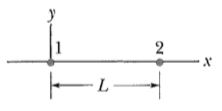
\includegraphics[width=0.30\textwidth]{./images/problems/lect01_3charges_0_net_force_on_third.png}
  \end{center}
\end{blockexmplque}

\vspace{0.2cm}

There is no equilibrium position for $q_3$ between the two fixed charges,
because it is being pulled by one and pushed by the other
(since $q_1$ and $q_2$ have different signs).
In this region, the two forces on q3 ($\vec{F}_{31}$ and $\vec{F}_{32}$)
have components that cannot cancel.

\end{frame}

%
%
%

\begin{frame}{Worked example: Equilibrium position of charge}

  For the same reason, there are no equilibrium positions off-axis
  (with the axis defined as that which passes through the two fixed charges),
  and therefore y=0.\\
  \vspace{0.3cm}

  On the semi-infinite region of the axis that is nearest $q_2$
  and furthest from $q_1$ an equilibrium position for $q_3$ cannot be found
  because $|q_1| < |q_2|$ and the magnitude of force exerted by $q_2$
  is everywhere (in that region) stronger than that exerted by $q_1$ on $q_3$.\\
  \vspace{0.3cm}

  Thus, we must look in the semi-infinite region of the axis which is nearest
  $q_1$ and furthest from $q_2$ (x$<$0).

\end{frame}

%
%
%

\begin{frame}{Worked example: Equilibrium position of charge}

  In that region, the net force on $q_3$ has magnitude which is given by:
  \begin{equation*}
     F_{3} = \left\rvert
               \frac{1}{4\pi\epsilon_0} \frac{|q_1 q_3|}{|x|^2} -
               \frac{1}{4\pi\epsilon_0} \frac{|q_2 q_3|}{(L+|x|)^2}
              \right\rvert
  \end{equation*}

  Setting $F_{3}$ equal to zero, the above expression yields:
  \begin{equation*}
    \frac{|q_1|}{|x|^2} - \frac{|q_2|}{(L+|x|)^2} = 0 \Rightarrow
    \Big(\frac{L+|x|}{|x|} \Big)^{2} = \frac{|q_2|}{|q_1|} \Rightarrow
    \frac{L}{|x|} + 1 = \sqrt{\frac{|q_2|}{|q_1|}} \Rightarrow
  \end{equation*}

  \begin{equation*}
    |x| = \frac{L}{\sqrt{\frac{|q_2|}{|q_1|}} - 1} \Rightarrow
  \end{equation*}

  \begin{equation*}
    |x| = \frac{10\;cm}{\sqrt{\frac{|-3\;{\mu}C|}{|+1\;{\mu}C|}} - 1}
        = \frac{10\;cm}{\sqrt{3} - 1} \approx 13.66 \; cm
    \Rightarrow x = -13.66 \; cm
  \end{equation*}

\end{frame}

} %\problemslide

% ------------------------------------------------------------------------------

%
% Worked example :
%

{
\problemslide

\begin{frame}{Worked example: Field of two charged beads on ring}

\begin{blockexmplque}{Question}
  The figure below shows a plastic ring of radius $R$ = 50 cm.
  Two small charged beads are on the ring: Bead 1 of charge +2 $\mu$C
	is fixed in place at the left side;
	bead 2 of charge +6 $\mu$C can be moved along the ring.
	The two beads produce a net electric field of magnitude $E$ at the
	centre of the ring.
  At what (a) positive and (b) negative value of
	angle $\theta$ should bead 2 be positioned so that $E$ = 2 $\times$ 10$^{5}$ N/C?\\
  \begin{center}
      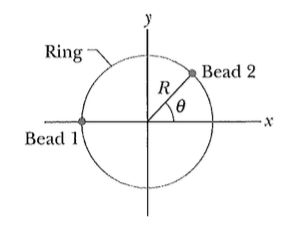
\includegraphics[width=0.34\textwidth]{./images/problems/lect01_ring_with_2_beads.png}
  \end{center}
\end{blockexmplque}

\end{frame}

%
%
%

\begin{frame}{Worked example: Field of two charged beads on ring}

  The net electric field components along x and y are
  \begin{equation*}
  	E_{x} = \frac{q_1}{4\pi\epsilon_0 R^2} - \frac{q_2 cos\theta}{4\pi\epsilon_0 R^2}
    \;\;\; and \;\;\;
  	E_{y} = - \frac{q_2 sin\theta}{4\pi\epsilon_0 R^2}
  \end{equation*}

  The magnitude of the net electric field is:
  \begin{equation*}
  	  E = \sqrt{E_{x}^2 + E_{y}^2} =
  		\sqrt{ (\frac{q_1}{4\pi\epsilon_0 R^2} - \frac{q_2 cos\theta}{4\pi\epsilon_0 R^2})^2 +
  					 (-\frac{q_2 sin\theta}{4\pi\epsilon_0 R^2})^2 }
  \end{equation*}
  \begin{equation*}
  		 = \frac{1}{4\pi\epsilon_0 R^2}
  			 \sqrt{ (q_1 - q_2 cos\theta)^2 + (q_2 sin\theta)^2 }
  \end{equation*}
  \begin{equation*}
  	    = \frac{1}{4\pi\epsilon_0 R^2}
  		    \sqrt{ q_1^2 + q_2^2 cos^2\theta + q_2^2 sin^2\theta - 2 q_1 q_2 cos\theta }
  \end{equation*}
  \begin{equation*}
  			= \frac{1}{4\pi\epsilon_0 R^2}
  			    \sqrt{ q_1^2 + q_2^2 - 2 q_1 q_2 cos\theta }
  \end{equation*}

\end{frame}

%
%
%

\begin{frame}{Worked example: Field of two charged beads on ring}

  Therefore:
  \begin{equation*}
      (E 4\pi\epsilon_0 R^2)^2 = q_1^2 + q_2^2 - 2 q_1 q_2 cos\theta \Rightarrow
      cos\theta = \frac{q_1^2 + q_2^2 - E^2 (4\pi\epsilon_0)^2 R^4}{2 q_1 q_2}
  \end{equation*}

  Substituting
  $E$ = 2 $\times$ 10$^{5}$ N/C
  $q_1$ = 2 $\times$10$^{-6}$ C,
  $q_2$ = 6 $\times$10$^{-6}$ C, and
  $R$ = 0.5 m,
  in the equation above, we have:

  \begin{equation*}
    \small
      cos\theta =
  		  \frac{(2 \times 10^{-6} \; C)^2 + (6 \times 10^{-6} \; C)^2 -
  			      (\frac{2 \times 10^{5} \; N/C}{8.99 \times 10^{9} \; N \cdot m^2/C^2})^2 (0.5 \; m)^4}
  					 {2 (2 \times 10^{-6} \; C) (6 \times 10^{-6} \; C)} \Rightarrow
  \end{equation*}

  \begin{equation*}
  		cos\theta \approx
  			 \frac{3}{8} = 0.375 \Rightarrow
  		\theta \approx \pm 68^{o}
  \end{equation*}

\end{frame}

} %\problemslide

% ------------------------------------------------------------------------------

%
% Worked example :
%

{
\problemslide

\begin{frame}{Worked example: $\vec{E}$ at centre of curvature of bent rod}

\begin{blockexmplque}{Question}

  \begin{columns}
    \begin{column}{0.60\textwidth}
      The figure on the right shows a plastic rod with total charge -$Q$ uniformly
      distributed along the rod. It is bent in a 120$^o$ circular arc of radius $R$
      and symmetrically placed across an x axis with the origin at the
      centre of curvature P of the rod.
    \end{column}
    \begin{column}{0.40\textwidth}
      \begin{center}
          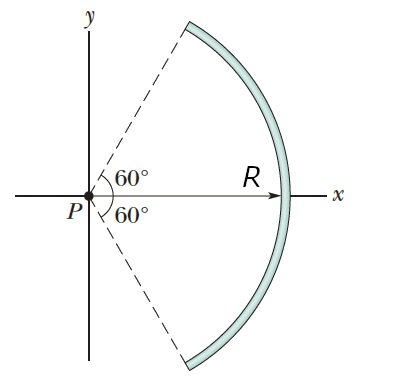
\includegraphics[width=0.95\textwidth]{./images/problems/lect01_plastic_rod_bent_circular_arc.png}
      \end{center}
    \end{column}
  \end{columns}
  \vspace{0.2cm}
  Show that the electric field $\vec{E}$, due to the rod, at point P is:
  \begin{equation*}
  		 \vec{E} = \frac{3\sqrt{3}Q}{8\pi^2 \epsilon_0 R^2} \hat{x}
  \end{equation*}
\end{blockexmplque}

\end{frame}

%
%
%

\begin{frame}{Worked example: $\vec{E}$ at centre of curvature of bent rod}

The electric field $\vec{E}$ at the point $\vec{r}$, due to a continuous
distribution of charge, is given by:
\begin{equation*}
  \vec{E}(\vec{r}) = \frac{1}{4\pi\epsilon_0}
   \int \frac{dq(\pvec{r}')}{|\vec{r}-\pvec{r}'|^3} (\vec{r}-\pvec{r}')
\end{equation*}

Taking the point $P$ to be at the origin of the coordinate system,
we have $\vec{r}=\vec{0}$,
while for the vector $\pvec{r}'$ pointing to charge $dq$
at an arbitrary point on the plastic rod (circular arc of radius $R$)
we can write $|\pvec{r}'|=R$ and $\pvec{r}'=R\hat{r}$.
Therefore, the above expression for $\vec{E}$ becomes:
\begin{equation*}
  \vec{E} = - \frac{1}{4\pi\epsilon_0 R^2}
   \int dq(\pvec{r}') \hat{r}
\end{equation*}

The infinitesimal charge $dq$ at position $\pvec{r}'$ can be expressed as:
\begin{equation*}
   dq(\pvec{r}') = \lambda d\ell
\end{equation*}

where $\lambda$ is the charge density.

\end{frame}

%
%
%

\begin{frame}{Worked example: $\vec{E}$ at centre of curvature of bent rod}

Considering that the charge is distributed
over a third of the circumference of a circle of radius $R$,
$\lambda$ is given by:
\begin{equation*}
   \lambda = \frac{-Q}{2\pi R/3} = -\frac{3Q}{2\pi R}
\end{equation*}

The element $d\ell$ is:
\begin{equation*}
   d\ell = R d\theta
\end{equation*}

Therefore, $dq$ can be written as:
\begin{equation*}
   dq(\pvec{r}') = -\frac{3Q}{2\pi} d\theta
\end{equation*}

Substituting $dq$ into the earlier expression for $\vec{E}$, we find:
\begin{equation*}
  \vec{E} =
   -\frac{1}{4\pi\epsilon_0 R^2} \Big(-\frac{3Q}{2\pi}\Big) \int_{-\pi/3}^{\pi/3} d\theta \hat{r} =
   \frac{3Q}{8\pi^2\epsilon_0 R^2} \int_{-\pi/3}^{\pi/3} d\theta \hat{r}
\end{equation*}

\end{frame}

%
%
%

\begin{frame}{Worked example: $\vec{E}$ at centre of curvature of bent rod}

The vector $\hat{r}$ is written in cartesian coordinates as:
\begin{equation*}
  \hat{r} = cos\theta \hat{x} + sin\theta \hat{y}
\end{equation*}

Substituting in the previous expression for $\vec{E}$, we have:
\begin{equation*}
  \vec{E} =
   \frac{3Q}{8\pi^2\epsilon_0 R^2}
   \Big\{ \hat{x} \int_{-\pi/3}^{\pi/3} cos\theta d\theta +
          \hat{y} \int_{-\pi/3}^{\pi/3} sin\theta d\theta
   \Big\} \Rightarrow
\end{equation*}

\begin{equation*}
  \vec{E} =
   \frac{3Q}{8\pi^2\epsilon_0 R^2}
   \Big\{ \hat{x} sin\theta \Big\rvert_{-\pi/3}^{\pi/3} -
          \hat{y} cos\theta \Big\rvert_{-\pi/3}^{\pi/3}
   \Big\} \Rightarrow
\end{equation*}

\begin{equation*}
  \vec{E} =
   \frac{3Q}{8\pi^2\epsilon_0 R^2}
   \Big\{ \hat{x} \Big( \frac{\sqrt{3}}{2} - (-\frac{\sqrt{3}}{2}) \Big) -
          \hat{y} \Big( \frac{1}{2} - \frac{1}{2} \Big)
   \Big\} \Rightarrow
\end{equation*}

\begin{equation*}
  \vec{E} =
   \frac{3\sqrt{3}Q}{8\pi^2\epsilon_0 R^2} \hat{x}
\end{equation*}

\end{frame}

} %\problemslide

% ------------------------------------------------------------------------------

%
% Worked example :
%

{
\problemslide


\begin{frame}{Worked example: $\vec{E}$ at centre of square formed by charges}

\begin{blockexmplque}{Question}

  \begin{columns}
    \begin{column}{0.65\textwidth}
      In the figure on the right, eight particles form a square in which distance
      $d$ is 2 cm.\\
      The charges are:
      $q_1$=+3$e$, $q_2$=+$e$, $q_3$=-5$e$, $q_4$=-2$e$,
      $q_5$=+3$e$, $q_6$=+$e$, $q_7$=-5$e$, and $q_8$=+$e$.\\
      In unit vector notation, what is the net electric field at the square's centre?
    \end{column}
    \begin{column}{0.35\textwidth}
      \begin{center}
          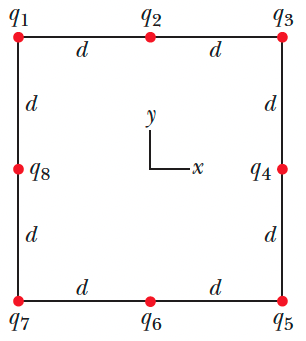
\includegraphics[width=0.70\textwidth]{./images/problems/lect01_8_charges_on_square.png}
      \end{center}
    \end{column}
  \end{columns}
\end{blockexmplque}

The total electric field $\vec{E}$ at the square's centre is computed,
using the superposition principle, as:
\begin{equation*}
  \vec{E} = \sum_{i=1}^{8} \vec{E}_{i}
\end{equation*}
where $\vec{E}_{i}$ is the electric field produced by charge $q_i$ ($i$=1,...,8).

\end{frame}

%
%
%

\begin{frame}{Worked example: $\vec{E}$ at centre of square formed by charges}


We note that, for the given charges, the electric fields along the diagonals
cancel out:
\begin{equation*}
  \vec{E}_{1} + \vec{E}_{5} = \vec{0}
\end{equation*}

\begin{equation*}
  \vec{E}_{3} + \vec{E}_{7} = \vec{0}
\end{equation*}

The remaining contributions to the total electric field are:
\begin{equation*}
  \vec{E}_4 =
    \frac{q_4}{4\pi\epsilon_0 d^2} \hat{x} =
    \frac{2e}{4\pi\epsilon_0 d^2} \hat{x}
\end{equation*}

\begin{equation*}
  \vec{E}_8 =
    \frac{q_8}{4\pi\epsilon_0 d^2} \hat{x} =
    \frac{e}{4\pi\epsilon_0 d^2} \hat{x}
\end{equation*}

Therefore, total electric field is given by:
\begin{equation*}
  \vec{E} =
    \frac{2e}{4\pi\epsilon_0 d^2} \hat{x} +
    \frac{e}{4\pi\epsilon_0 d^2} \hat{x} =
    \frac{3e}{4\pi\epsilon_0 d^2} \hat{x}
\end{equation*}


\end{frame}


} %\problemslide

% ------------------------------------------------------------------------------

%
% Programming task
%

{
\programmingslide

%
%
%

\begin{frame}{PHYS201 scientific programming task for Lecture \thislecture}

{\small

Write a program that:
\begin{itemize}
{\scriptsize
  \item {\bf Can read an arbitrary distribution of N discrete charges (in 2-D)},\\
        e.g. by accepting as input a text file with N rows, where the $i^{th}$
        row contains the coordinates $x_i$, $y_i$ in m, and the charge $q_i$ in C.
  \item {\bf Allows you to visualise the input charge distribution},\\
        e.g using appropriately-positioned circles whose color or size represents amount of charge.
  \item {\bf Allows you to visualise the electric field lines}
        in the vicinity of the charge distrubution.\\
}
\end{itemize}

\vspace{0.2cm}
Test your program, reproducing some of the simpler field maps shown before.\\

}

\end{frame}

} % programming
